\title{AVL Trees  - Recitation 7} 
\documentclass{article}


\usepackage[utf8]{inputenc}
\usepackage[a4paper, total={6in, 9in}]{geometry}
\usepackage{braket}
\usepackage{xcolor}
\usepackage{amsmath}
\usepackage{amsfonts}
\usepackage{tikz}
\usepackage{svg}
\usepackage{graphicx}
\usepackage{media9}
\usepackage{float}
\usetikzlibrary{calc}
\usepackage{array}
\usepackage[ruled,vlined,linesnumbered]{algorithm2e}

\usepackage[
backend=biber,
style=alphabetic,
sorting=ynt
]{biblatex}



\newcommand{\commentt}[1]{\textcolor{blue}{ \textbf{[COMMENT]} #1}}
\newcommand{\ctt}[1]{\commentt{#1}}
\newcommand{\prb}[1]{ \mathbf{Pr} \left[ {#1} \right]}
\newcommand{\onotation}[1]{\(\mathcal{O} \left( {#1}  \right) \)}
\newcommand{\ona}[1]{\onotation{#1}}
\newcommand{\nvar}[2]{ \( #1_{1}, #1_{2} ... #1_{#2}  \) }
%\newenvironment{proof}[0]{\paragraph{Proof.}}{}
%\newenvironment{remark}[0]{\textit{remark}}{}
\newenvironment{cor}[0]{\paragraph{Corollary.}}{}
\newenvironment{example}[0]{\paragraph{Example.}}{}
%\newenvironment{thm}[0]{\paragraph{Theorem.}}{}
\newtheorem{prop}{Proposition}
\newtheorem{ex}{Exercise}
\newtheorem{sol}{Solution}
\newtheorem{theorem}{Theorem} 		
\newtheorem{thm}{Theorem}[section]
\newtheorem{conj}[thm]{Conjecture} 	
\newtheorem{lemma}[thm]{Lemma}
\newtheorem{corollary}[thm]{Corollary} 
\newtheorem{claim}[thm]{Claim}
\newtheorem{proposition}[thm]{Proposition}
\newtheorem{definition}{Definition} 
\newtheorem{remark}{Remark}
 


% \addbibresource{sample.bib} %Import the bibliography file
\begin{document}    
\maketitle

%\begin{abstract}
%\begin{abstract}
    In this recitation we will review the new data structures you've seen - Binary
    search trees, and specifically AVL trees. We'll revise the different
    operations, go over the important concepts of balance factor and
    rotations and see some examples. If there's time left - we will prove
    that the height of an AVL tree is $O(\log(n))$.
%\end{abstract}
    
\section{AVL trees}
    Reminders:
    \begin{defbox}{Binary Tree.}
        A binary tree is a tree $(T,r)$ with $r\in V$, such that $\deg(v)
            \leq 2$ for any $v\in V$.
    \end{defbox}
    \begin{defbox}{Height.} A tree's height $h(T)$ (sometimes $h(r)$) is defined to be the
    length of the
    longest
    simple path from $r$ to a leaf.
    \end{defbox}
    \begin{defbox}{ Binary Search Tree. } A binary search tree is a binary tree $(T,r)$ such that for any
    node $x$ (root of a subtree) and a node in that subtree $y$:
    \begin{enumerate}
        \item if $y$ is in the left subtree of $x$ then $y.key \leq x.key$
        \item if $y$ is in the right subtree of $x$ then $x.key < y.key$
    \end{enumerate}
        Note that this is a (relatively) local property.
    \end{defbox}
For example:\\
    \begin{center}
        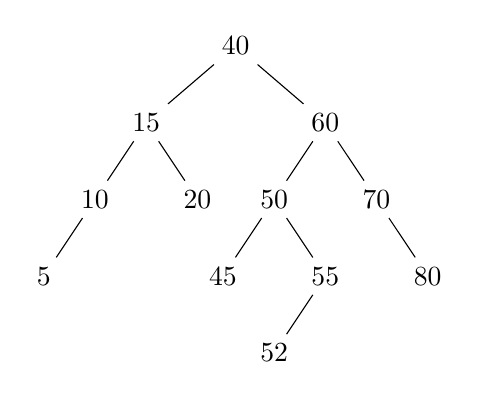
\begin{tikzpicture}[ level distance=1.5cm,
        level 1/.style={sibling distance=3.5cm},
        level 2/.style={sibling distance=2cm}, scale=.65]
            \node {40}
                child{node{15}
                        child{node{10} child{node{5}} child{node{} edge from parent
            [draw=none]}}
                        child{node{20}}}
                child{node{60}
                        child{node{50}
                                child{node{45}}
                                child{node{55}
                                        child{node{52}}
                                        child{node{} edge from parent [draw=none]}
                                }
                                }
                        child{node{70} child{node{} edge from parent [draw=none]}
                                child{node{80}}}
            };
    \end{tikzpicture}
    \end{center}
\begin{remark} Go over the properties, calculate the tree's height. Make sure you
understand the definitions!
\end{remark}

Last time, we have seen some operations that can be performed on BSTs, and
proved correctness for some of them. These were: $Search(x), Min(T), Max(T), Pred(x), Succ(x),
Insert(x), Delete(x)$. All of these operations take $O(h(T))$ in the worst case.\\

The main two operations that may cause problems are $Insert$ and $Delete$, as
they change the tree's height (consider inserting $81,82,83,84$ to our
working example).
To address this problem, we introduce another filed: for each node $v$ add a
field of $h(v)$ = the height of the subtree who's root is $v$. This allows us
to maintain the AVL property:
\begin{defbox}{AVL Tree.} An AVL tree is a balanced BST, such that for any node $x$, it's left
    and right subtrees' height differ in no more than $1$. In other words:
        $$|h(left(x)) - h(right(x))|\leq 1$$
    \end{defbox}
    This field allows us to calculate the Balance Factor for each node in $O
    (1)$:
    \begin{defbox}{Balance Factor.} For each node $x\in T$, it's Balance Factor is defined 
    $$hd
    (x) := h(left(x)) - h(right(x))$$ In AVL trees, we would like to maintain
    $|hd(x)| \leq 1$
    \end{defbox}
\begin{example} For our working example, the node $60$'s $hd$ is $h(50) - h
(70) = 1$, and $hd(50) = h(45)- h(55) = -1$. You can check and see that this
is an AVL tree.
\end{example}
So to make sure that we can actually maintain time complexity $O(\log(n))$, 
we'd want to:
\begin{enumerate}
    \item Show that for an AVL tree, $h(T) = \theta(log(n))$ (If there's time
    left)
    \item See how to correct violations in AVL property - using \textbf{rotations}
    \item See how to $Delete$ and $Insert$, while maintaining the height field.
\end{enumerate}

%\newpage
\subsection{Rotations}
\begin{figure}[h]
  \centering
\includegraphics[scale=.3]{Recitations/rotations.png}\\
\end{figure}
Rotations allow us to maintain the AVL property, in $O(1)$ time (you've
discussed this in the lecture - changing subtree's roots).
In
this
schematic
representation of rotations, $x,y$ are nodes and $\alpha,\beta,\gamma$ are subtrees.
Note that the BST property is maintained! \\

%\includegraphics[scale=.5]{Recitations/rotationEg.png}

The Balance factor allows us to identify if the AVL property was violated, and moreover -
the exact values of the bad Balance factors will tell us which rotations to do to fix
this:\\
Taken from last year's recitation:\\
\includegraphics[scale=.6]{Recitations/violations.png}

Let's analyze one of these cases:\\
\begin{example} Let's see why R rotation Fixes LL violation:\\
\begin{figure}[h]
  \centering
\includegraphics[scale=.5]{Recitations/LLviolation.jpg}\\
This is the general form of LL violations.
\end{figure}

Analyze the heights of subtrees. Denote $h$ the height of $A_L$ before
inserting $v$. So $A_R$'s height has to also be $h$.
If it's height was $h+1$, the insertion wouldn't have created a violation in
$B$ ($A$'s height would have stayed the same). If it was $h-1$, the violation
would've appeared first in $A$ (not in $B$). Thus, $A$'s height is $h+1$.
$B_R$'s height is also $h$: If it was $h+1$ or $h+2$, no violation in $B$ had
occurred.

After the rotation, the tree looks like this:
\begin{figure}[h]
  \centering
  \includegraphics[scale=.9]{Recitations/LLviolationfix.jpg}
\end{figure}
So all the nodes here maintain AVL property; why is it maintained in general?
\end{example}\\
Detect the violation in the following tree, and perform the necessary rotations:\\
\begin{figure}[h]
  \centering
  \begin{subfigure}[b]{0.31\textwidth}
            \begin{tikzpicture}[ level distance=1.5cm,
        level 1/.style={sibling distance=3.5cm},
        level 2/.style={sibling distance=2cm}, scale=.65]
            \node {15}
	    child{node{5} child{node{3}} child{node{12}  child{node{10}
            child{node{6}} child{node{} edge from parent [draw = none]}}
            child{node{13}}}} child{node{20} child{node{18}} child{node{23}}}
            ;
    \end{tikzpicture}
  \end{subfigure}
\begin{subfigure}[b]{0.31\textwidth}
        \begin{tikzpicture}[ level distance=1.5cm,
        level 1/.style={sibling distance=3.5cm},
        level 2/.style={sibling distance=2cm}, scale=.65]
            \node {15}
	    child{node{} child{node{3}} child{node{10}
            child{node{6}} child{node{12} child{node{} edge
            from parent [draw = none]} child{node{13}} }}
            }
             child{node{20} child{node{18}} child{node{23}}}
            ;
    \end{tikzpicture}
  \end{subfigure}
\begin{subfigure}[b]{0.31\textwidth}
  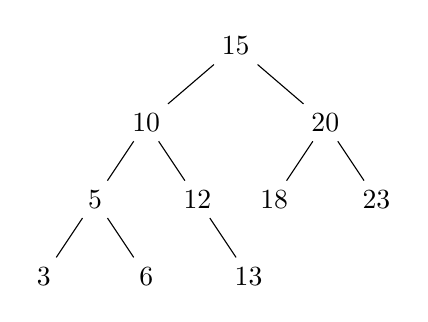
\begin{tikzpicture}[ level distance=1.5cm,
        level 1/.style={sibling distance=3.5cm},
        level 2/.style={sibling distance=2cm}, scale=.65]
            \node {15}
                child{node{10} child{node{5} child{node{3}} child{node{6}}
            } child{node{12}
            child{node{} edge from parent [draw = none]} child{node{13}}}}
             child{node{20} child{node{18}} child{node{23}}}
            ;
    \end{tikzpicture}

\end{subfigure}
  \caption{ 
The first node in which a violation occurred is $5$, this is an RL violation.
Perform R rotation on the right child. Then perform L rotation on the root of the relevant subtree ($5$):
}
\end{figure}
\subsection{Delete, Insert.}
The principles of the $Delete$ and $Insert$ operations are the same as in
regular BST, but we will need to rebalance the tree in order to preserv AVL
property.
A single insertion or deletion may change the height difference of subtrees
by at most 1, and might affect only the subtrees with roots along the path
from $r$ to the point of insertion/ deletion.
More concretely - we will add a recursive operation of traversing the tree
"back up" and checking violations. Had we found one - we'll fix it using
rotations. Since rotations can be done in $O(1)$, the entire correction
process will take $O(\log(n))$, so we maintain a good time complexity.


\begin{algbox}{AVL Insert(r,x)}
  \begin{algorithm}[H]
    Call Insert $(r,x)$ // (The standart insertion routine for BST) \\  
    Let $p$ be the new node appended to the tree. \\
    \While{ $p$.parent $\neq \emptyset $ } {
      Check in which of the four states we are. \\ 
      Apply the right rotation. \\ 
      Update the height of each toched vertex  \\
      $p \leftarrow$ $p$.parent \\  
    }
  \end{algorithm}
\end{algbox}


\iffalse
\newpage
\subsection{Delete, Insert}
The principles of the $Delete$ and $Insert$ operations are the same as in
regular BST, but we will need to rebalance the tree in order to preserv AVL
property.
A single insertion or deletion may change the height difference of subtrees
by at most 1, and might affect only the subtrees with roots along the path
from $r$ to the point of insertion/ deletion.
More concretely - we will add a recursive operation of traversing the tree
"back up" and checking violations. Had we found one - we'll fix it using
rotations. Since rotations can be done in $O(1)$, the entire correction
process will take $O(\log(n))$, so we maintain a good time complexity.
\subsubsection{Delete}
This is the regular BST delete, we will need to traverse up the
tree and detect violations (if occurred).\\
\includegraphics[scale=.6]{Recitations/DeleteBST.jpg}\\
\begin{remark} Go over the procedure quickly - explain the 3 cases - no
children, 1 child (easy) and 2 children (using successor).
\end{remark}
\begin{example}\\
    Delete $20$ from the tree in the beginning of the recitation:\\
    \includegraphics[scale=.3]{Recitations/DeleteEx.jpg}
\end{example}
%    Consider the original BST we looked at:\\
%
%\begin{tikzpicture}[ level distance=1.5cm,
%        level 1/.style={sibling distance=3.5cm},
%        level 2/.style={sibling distance=2cm}, scale=.65]
%            \node {40}
%                child{node{15}
%                        child{node{10} child{node{5}} child{node{} edge from parent
%            [draw=none]}}
%                        child{node{20}}}
%                child{node{60}
%                        child{node{50}
%                                child{node{45}}
%                                child{node{55}
%                                        child{node{52}}
%                                        child{node{} edge from parent [draw=none]}
%                                }
%                                }
%                        child{node{70} child{node{} edge from parent [draw=none]}
%                                child{node{80}}}
%            };
%    \end{tikzpicture}
%
%Let's $Insert(4)$:\\
%
%\begin{tikzpicture}[ level distance=1.5cm,
%        level 1/.style={sibling distance=3.5cm},
%        level 2/.style={sibling distance=2cm}, scale=.65]
%            \node {40}
%                child{node{15}
%                        child{node{(-2)10} child{node{(-1)5}child{node{4}}
%            child{node{} edge
%            from
%            parent
%            [draw = none]} }
%            child{node{} edge from
%            parent
%            [draw=none]}}
%                        child{node{20}}}
%                child{node{60}
%                        child{node{50}
%                                child{node{45}}
%                                child{node{55}
%                                        child{node{52}}
%                                        child{node{} edge from parent [draw=none]}
%                                }
%                                }
%                        child{node{70} child{node{} edge from parent [draw=none]}
%                                child{node{80}}}
%            };
%    \end{tikzpicture}\\
%
%So we need to fix LL violation, this is by preforming R rotation of the root
%of the subtree in which the violation first appeared: \\
%
%\begin{tikzpicture}[ level distance=1.5cm,
%        level 1/.style={sibling distance=3.5cm},
%        level 2/.style={sibling distance=2cm}, scale=.65]
%            \node {40}
%                child{node{15}
%                        child{node{(0)5} child{node{(0)4}} child{node{10}}
%             }
%                        child{node{20}}}
%                child{node{60}
%                        child{node{50}
%                                child{node{45}}
%                                child{node{55}
%                                        child{node{52}}
%                                        child{node{} edge from parent [draw=none]}
%                                }
%                                }
%                        child{node{70} child{node{} edge from parent [draw=none]}
%                                child{node{80}}}
%            };
%    \end{tikzpicture}
%\begin{remark}
%    RR rotations are symmetric
%\end{remark}
\subsubsection{Insert}
Once again - this is the regular BST insert, we will need to traverse up the
tree and detect violations (if occurred).\\
\includegraphics[scale=.6]{Recitations/InsertBST.jpg}\\
\begin{example}
    Insert $65$ tho the previous tree (after the deletion):\\
    \begin{tikzpicture}[ level distance=1.5cm,
        level 1/.style={sibling distance=3.5cm},
        level 2/.style={sibling distance=2cm}, scale=.65]
            \node{50} child{node{40} child{node{10} child{node{5}
            }child{node{15}}} child{node{45}}}
            child{node{60} child{node{55}
                                    child{node{52}} child{node{} edge from
                                                            parent [draw=none]}}
                                    child{node{70}
                                            child{node{} edge from parent
            [draw=none]} child{node{80}}}}

    \end{tikzpicture}\\
    So after the insertion:\\
        \begin{tikzpicture}[ level distance=1.5cm,
        level 1/.style={sibling distance=3.5cm},
        level 2/.style={sibling distance=2cm}, scale=.65]
            \node{50} child{node{40} child{node{10} child{node{5}
            }child{node{15}}} child{node{45}}}
            child{node{60} child{node{55}
                                    child{node{52}} child{node{} edge from
                                                            parent [draw=none]}}
                                    child{node{70}
                                            child{node{65}} child{node{80}}}}

    \end{tikzpicture}\\
    And no violation occurred.\\
    \newpage
\end{example}
\begin{example}
    Insert 53 to the previous tree:\\
    \begin{tikzpicture}[ level distance=1.5cm,
        level 1/.style={sibling distance=3.5cm},
        level 2/.style={sibling distance=2cm}, scale=.65]
            \node{50} child{node{40} child{node{10} child{node{5}
            }child{node{15}}} child{node{45}}}
            child{node{60} child{node{55}
                                    child{node{52} child{node{} edge from
            parent [draw=none]} child{node{53}}} child{node{}
            edge
            from
                                                            parent [draw=none]}}
                                    child{node{70}
                                            child{node{65}} child{node{80}}}}

    \end{tikzpicture}\\
    Detect LR violation in $55$: Perform $L$ rotation on $52$:\\
    \begin{tikzpicture}[ level distance=1.5cm,
        level 1/.style={sibling distance=3.5cm},
        level 2/.style={sibling distance=2cm}, scale=.65]
            \node{50} child{node{40} child{node{10} child{node{5}
            }child{node{15}}} child{node{45}}}
            child{node{60} child{node{55}
                                    child{node{53} child{node{52}}
            child{node{} edge from parent[draw=none]}}
            child{node{}
            edge
            from
                                                            parent [draw=none]}}
                                    child{node{70}
                                            child{node{65}} child{node{80}}}}

    \end{tikzpicture}\\
    perform $R$ rotation on $55$:\\
    \begin{tikzpicture}[ level distance=1.5cm,
        level 2/.style={sibling distance=3cm},
        level 1/.style={sibling distance=5cm},
        level 3/.style={sibling distance=1.5cm},scale=.65]
            \node{50} child{node{40} child{node{10} child{node{5}
            }child{node{15}}} child{node{45}}}
            child{node{60} child{node{53}
                                    child{node{52}}
            child{node{55}}}
                                    child{node{70}
                                            child{node{65}} child{node{80}}}}

    \end{tikzpicture}\\

\end{example}

\newpage
\fi
\subsection{Exam Question.}
Consider the following question form 2018 exam. 
\begin{figure}[h]
  \centering
  
\includegraphics[scale=0.8]{avl-q-exam.png}\\
\end{figure}



\begin{figure}[H]
  \begin{subfigure}[b]{0.49\textwidth}
    \paragraph{Solution.} 

How would look like an algorithm which compute the 'sumover' query? Or for given $x$ which vertics are the ones with a key less than $x$. 
Consdier the path $v_1,v_2,v_3...v_n$ on which the Search subroutine went over when looking for $x$. If $v_i$.key $ <  v_{i+1}$.key then it means that $x$ is 
greater then $v_{i}$.key. And therefore $x$ is also greater than all the keys in the left subtree of $v_{i}$.

\paragraph{}

Let's transform that insight into an 
Algorithm. Define for each vertex a field that stores the summation of all it's left subtree keys plus it's own key, Call it 'Leftsum'.  
Then computing the sumover query will be done by summing theose fields of the verteics in the right turn on the searching path. 
\end{subfigure} 
\hfill
\begin{subfigure}[b]{0.49\textwidth}
  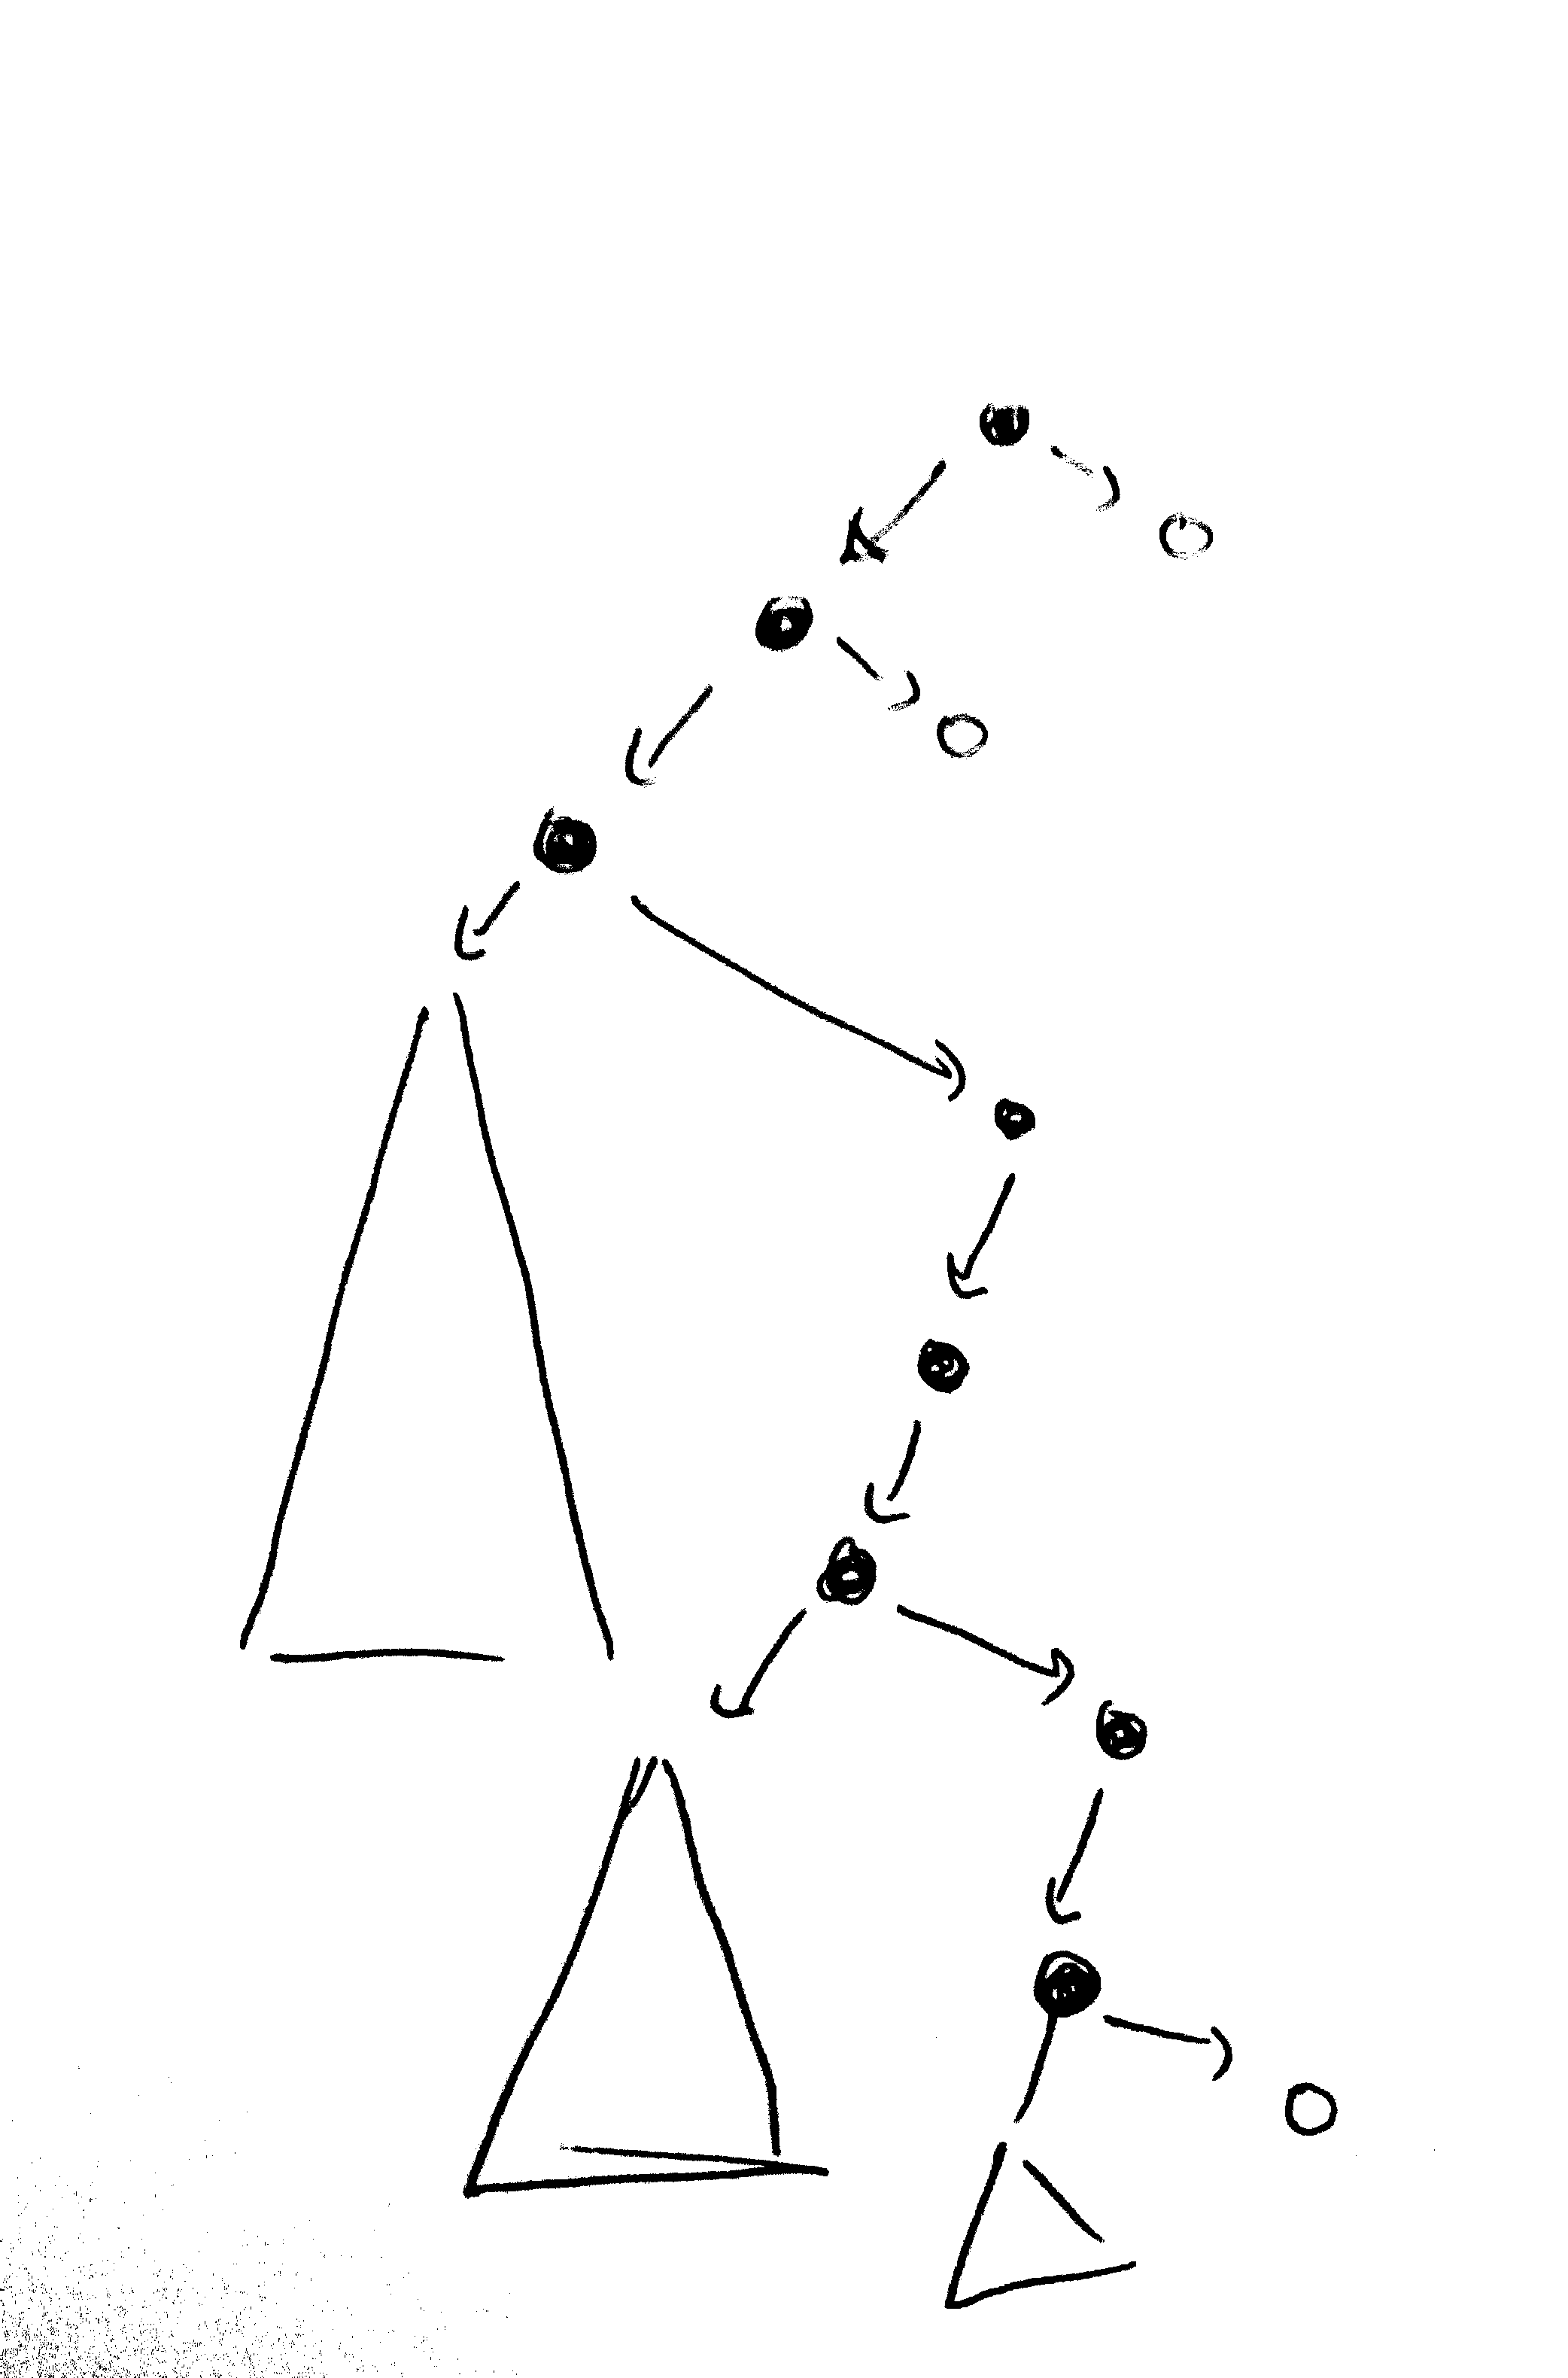
\includegraphics[scale=0.08]{oavl-q.png}
   \end{subfigure} 
   \hfill
\end{figure}


\begin{algbox}{Sumover($r$,$x$)}
  \begin{algorithm}[H]
    \If{ $r$ is None }{
      return $0$ 
    }\Else{
      \If{$x > r$.key }{
	return $r$.Leftsum + Sumover( $r$.right, $x$ )  
      }\Else{
      	return Sumover( $r$.left, $x$ )  
      }
    }
  \end{algorithm}
\end{algbox}

So it's left to show how one could maintain the tree and gurantee a logrithmic hieght. Consider a vertex $v$ and suppose that both
his direct children are correct AVL trees and also has the correct value at the Leftsum field. We know that:
\begin{enumerate}
  \item There is a rotaiton that blanced the tree at the cost of $O(1)$ time.
  \item All the descendants of $v$ distance at distance grater than $2$ form it will remain the same, in the sanse that 
    their subtree will not change. 
\end{enumerate}
Therefore we will have to recompute the Sumleft filed for only a $O(1)$ vertics (which are the children and the grandchildren of $v$ privews the rotation). 
Each of that compution could be done in $O(1)$ time. 


\begin{algbox}{AVL-Leftsum Insert(r,x)}
  \begin{algorithm}[H]
    Call Insert $(r,x)$ // (The standart insertion routine for BST) \\  
    Let $p$ be the new node appended to the tree. \\
    \While{ $p$.parent $\neq \emptyset $ } {
      Apply the right rotation. \\
      \For{ any vertex $v$ such that its pointers have changed, sorted by height } {
	$v$.Leftsum $\leftarrow$ $v$.key + $v$.left.Leftsum + $v$.left.right.Leftsum 		
      }
      $p \leftarrow$ $p$.parent \\  
    }
  \end{algorithm}
\end{algbox}

\paragraph{Running time.} The work is made over vertices along a single path, and on each vartics only $O(1)$ time 
is spent, Then we have that the total running time of the algorithm is proptional to the tree hight. 
Combine the fact that we maintain tha AVL property it follows that the total time is $\Theta\left( \log n \right)$.  




\section*{Appendix}
\subsection{AVL tree's height}
Let $n_h$ be the minimal number of nodes in an AVL tree of height
$h$.\\
\begin{thm}
    $n_h$ is strictly increasing in $h$.
\end{thm}
\begin{proof} Exercise.
\end{proof}
\begin{thm}
$n_{h} = n_{h-1} + n_{h-2} + 1$.
\end{thm}
\begin{proof}For an AVL tree of height $0$, $n_0 = 1$,
and of height $1$, $n_1 = 2 $ (by checking directly).\\
    Let's look at a minimal AVL tree of height $h$. By the AVL property, one
of it's subtrees is of height $h-1$ (WLOG - the left subtree) and by
minimality, it's left subtree has to have $n_{h-1}$ nodes. $T$'s right subtree
thus has to be of height $h-2$: It can't be of height $h-1$: $n_{h-1} >
n_{h-2}$ by previous theorem, and if the right subtree is of height $h-1$ -
we could switch it with an AVL tree of height $h-2$, with less nodes - so
less nodes in $T$, contradicting minimality. So the right subtree has
$n_{h-2}$ nodes (once again, by minimality), and thus the whole tree has
    $n_{h} = n_{h-1} + n_{h-2} + 1$ (added the root) nodes.
\end{proof}
\begin{cor}$n_h > 2n_{h-2} + 1$
\end{cor}
\begin{cor}$h = O(\log(n))$
\end{cor}
\begin{proof}
    Assume $k$ is even (why can we assume that?).
    It can be shown by induction that:
    \[
        n_h>2n_{h-2}+1>2(2n_{h-4}+1)+1=4n_{h-4}+(1+2)\ldots >
        2^{\frac{h}{2}}+\sum_{i=0}^{\frac{h}{2}-1}
        2^i=\sum_{i=1}^{\frac{h}{2}}2^i = \frac{2^\frac{h}{2} - 1}{2-1} =  2^{\frac{h}{2}} - 1
    \]
    So $n_h \geq 2^{\frac{h}{2}} - 1$, thus
    \[
        h\leq 2\log(n_h + 1)
    \]
    and for generall AVL tree with $n$ nodes and height $h$:
    \[
         h\leq 2\log(n_h + 1) \leq 2\log(n + 1) = O(\log(n))
    \]
%    By $n_h$'s minimality:
%    $$n \geq n_h \geq F_h = C (\varphi^h - (-\varphi)^h) \geq
%    \tilde{C}\varphi^h$$
%    Thus
%    $h \leq \frac{1}{\tilde{C}} \log_{\varphi}(n)$
\end{proof}
\begin{remark}
    In fact, one can show that $n_h > F_h$ and $F_h$ is the $h$'th Fibonacci
    number. Recall that $F_h = C(\varphi^h - (\psi)^h)$, and this gives a
    tighter bound on $n_h$.
\end{remark}

% \printbibliography 
\end{document}


